\chapter{Analyse et Conception}

\section{Introduction}

Ce chapitre présente la démarche d'analyse et de conception adoptée pour le développement de
LudoHeritage. Il recense les besoins fonctionnels et non-fonctionnels identifiés, décrit
l'architecture choisie, présente le modèle de données et explique les choix de conception
de l'interface utilisateur.

% ─────────────────────────────────────────────────────────────────────────────
\section{Analyse des besoins}
% ─────────────────────────────────────────────────────────────────────────────

\subsection{Identification des acteurs}

La plateforme LudoHeritage cible deux types d'acteurs principaux~:

\begin{itemize}
    \item \textbf{L'utilisateur authentifié~:} toute personne disposant d'un compte. Il peut
          consulter le catalogue, interagir avec LudoBot, participer au forum, passer des quiz
          et gérer son profil.

    \item \textbf{L'utilisateur non authentifié~:} un visiteur qui peut voir la page d'accueil
          mais qui doit créer un compte pour accéder aux fonctionnalités complètes.
\end{itemize}

\subsection{Besoins fonctionnels}

Les fonctionnalités attendues par les utilisateurs sont organisées en six modules~:

\begin{table}[H]
\centering
\renewcommand{\arraystretch}{1.4}
\begin{tabularx}{\textwidth}{>{\bfseries}p{3.5cm} X}
\toprule
\textbf{Module} & \textbf{Fonctionnalités} \\
\midrule
Authentification
    & Créer un compte avec validation d'e-mail et confirmation de mot de passe.
      Se connecter de façon sécurisée. Compléter un questionnaire d'intégration (onboarding)
      pour personnaliser l'expérience. \\
\midrule
Catalogue des jeux
    & Parcourir les 20 jeux du catalogue. Filtrer par région, période, type et niveau.
      Rechercher par nom, alias, pays ou mécanique.
      Consulter la fiche détaillée de chaque jeu (règles, histoire, culture, mécaniques). \\
\midrule
Visualisation
    & Explorer les jeux sur une carte SVG mondiale interactive.
      Visualiser l'histoire des jeux sur une frise chronologique cliquable.
      Filtrer le catalogue en cliquant sur un continent ou une période. \\
\midrule
Outils pédagogiques
    & Comparer deux jeux côte à côte (caractéristiques et ludèmes communs).
      Jouer à un quiz de 10 questions aléatoires sur les jeux.
      Consulter un classement des meilleurs scores.
      Jouer à l'Awale directement dans le navigateur. \\
\midrule
LudoBot (IA)
    & Poser des questions en langage naturel sur les jeux.
      Recevoir des recommandations personnalisées selon son profil.
      Obtenir des explications de règles, des conseils stratégiques et des informations
      culturelles. \\
\midrule
Communauté \& Profil
    & Publier des messages dans le forum et lier un jeu à sa publication.
      Liker et commenter les publications des autres.
      Gérer ses favoris et ses préférences.
      Consulter son historique de jeux récemment explorés et ses succès débloqués. \\
\bottomrule
\end{tabularx}
\caption{Besoins fonctionnels par module}
\label{tab:fonctionnels}
\end{table}

\subsection{Besoins non-fonctionnels}

Au-delà des fonctionnalités, plusieurs exigences de qualité ont guidé la conception~:

\begin{itemize}
    \item \textbf{Performance~:} les pages doivent se charger en moins de 2 secondes sur une
          connexion standard. Le catalogue de 20 jeux doit être disponible immédiatement, même
          si MongoDB est hors ligne (données de secours en mémoire).

    \item \textbf{Sécurité~:} les mots de passe sont hashés avec BCrypt. Les entrées utilisateur
          sont validées côté backend (\texttt{@Valid}). Un gestionnaire global d'exceptions
          retourne des messages d'erreur structurés.

    \item \textbf{Responsivité~:} l'interface s'adapte aux écrans de toutes tailles grâce à une
          conception \textit{mobile-first} en CSS Grid et Flexbox.

    \item \textbf{Maintenabilité~:} le backend suit une architecture en couches (contrôleurs,
          services, repositories). Le frontend est organisé en composants React réutilisables.

    \item \textbf{Accessibilité culturelle~:} le contenu est sélectionné pour être compatible avec
          les valeurs culturelles et religieuses du public cible (aucun jeu à contenu haram).
\end{itemize}

% ─────────────────────────────────────────────────────────────────────────────
\section{Conception}
% ─────────────────────────────────────────────────────────────────────────────

\subsection{Diagramme de cas d'utilisation}

Le diagramme de cas d'utilisation donne une vue d'ensemble des actions que chaque type
d'utilisateur peut réaliser sur la plateforme. Il permet de visualiser le périmètre du
système et les relations entre les acteurs et les fonctionnalités, avant même de commencer
à développer.

\begin{figure}[H]
    \centering
    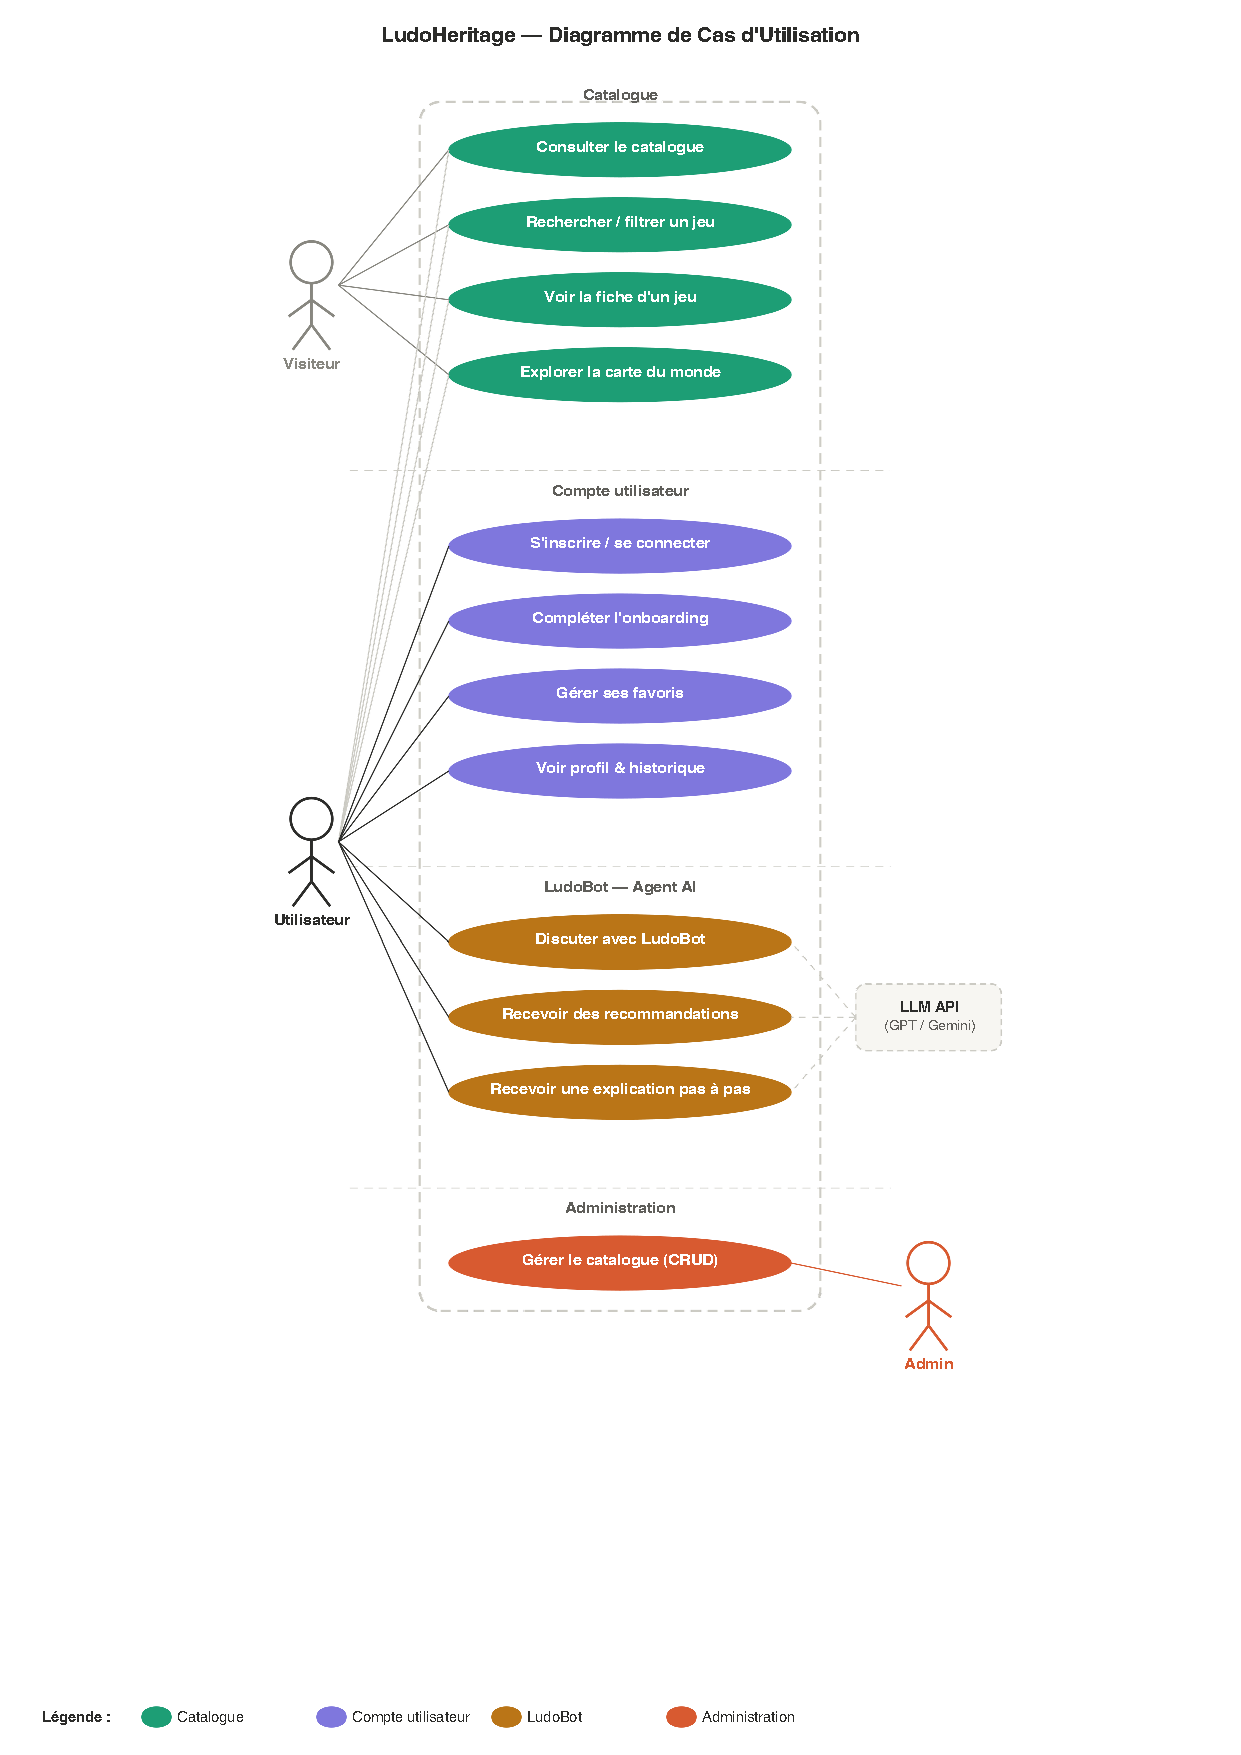
\includegraphics[width=\textwidth]{uml_usecase.pdf}
    \caption{Diagramme de cas d'utilisation -- LudoHeritage}
    \label{fig:usecase}
\end{figure}

\subsection{Description détaillée des cas d'utilisation}

Les tableaux suivants décrivent les scénarios les plus importants de la plateforme,
étape par étape, en précisant les conditions de départ, le déroulement normal et les
cas d'erreur possibles~:

\vspace{0.4cm}

\begin{table}[H]
\centering
\renewcommand{\arraystretch}{1.6}
\begin{tabular}{|p{4cm}|p{9.5cm}|}
\hline
\rowcolor{ludocolor!25}
\multicolumn{2}{|l|}{\textbf{UC1 -- S'inscrire et compléter l'intégration}} \\
\hline
Acteur principal & Visiteur \\
\hline
Préconditions & Aucune \\
\hline
Postconditions & Compte créé, préférences sauvegardées, utilisateur connecté \\
\hline
Déroulement normal &
1. Le visiteur clique sur « S'inscrire ». \newline
2. Il saisit son nom, son e-mail et un mot de passe. \newline
3. Il confirme son mot de passe. \newline
4. Le système vérifie les informations et crée le compte. \newline
5. L'utilisateur répond au questionnaire de bienvenue (niveau, préférences). \newline
6. LudoBot propose trois jeux correspondant à son profil. \\
\hline
Cas d'erreur & Si l'e-mail est déjà utilisé, un message d'erreur est affiché. \\
\hline
\end{tabular}
\caption{UC1 -- S'inscrire et compléter l'intégration}
\label{tab:uc1}
\end{table}

\vspace{0.3cm}

\begin{table}[H]
\centering
\renewcommand{\arraystretch}{1.6}
\begin{tabular}{|p{4cm}|p{9.5cm}|}
\hline
\rowcolor{ludocolor!25}
\multicolumn{2}{|l|}{\textbf{UC2 -- Voir la fiche détaillée d'un jeu}} \\
\hline
Acteur principal & Visiteur, Utilisateur \\
\hline
Préconditions & Un jeu est sélectionné dans le catalogue \\
\hline
Postconditions & La fiche complète du jeu est consultée \\
\hline
Déroulement normal &
1. L'utilisateur clique sur une carte de jeu. \newline
2. Le système affiche la fiche avec quatre onglets~: Aperçu, Règles, Histoire,
   Mécanique. \newline
3. L'utilisateur navigue entre les onglets selon son intérêt. \newline
4. Si le jeu est l'Awale, un onglet « Jouer » est disponible. \newline
5. L'utilisateur peut ajouter le jeu à ses favoris (s'il est connecté). \\
\hline
Cas d'erreur & Aucun (le catalogue est toujours disponible). \\
\hline
\end{tabular}
\caption{UC2 -- Voir la fiche détaillée d'un jeu}
\label{tab:uc2}
\end{table}

\vspace{0.3cm}

\begin{table}[H]
\centering
\renewcommand{\arraystretch}{1.6}
\begin{tabular}{|p{4cm}|p{9.5cm}|}
\hline
\rowcolor{ludocolor!25}
\multicolumn{2}{|l|}{\textbf{UC3 -- Discuter avec LudoBot pour une recommandation}} \\
\hline
Acteur principal & Utilisateur connecté \\
\hline
Préconditions & L'utilisateur est connecté et a complété l'intégration \\
\hline
Postconditions & LudoBot propose un jeu avec une explication \\
\hline
Déroulement normal &
1. L'utilisateur ouvre le panneau LudoBot. \newline
2. Il écrit par exemple « Recommande-moi un jeu ». \newline
3. LudoBot consulte le profil de l'utilisateur et le catalogue. \newline
4. LudoBot répond avec un jeu adapté et explique son choix. \newline
5. L'utilisateur peut poser d'autres questions pour affiner. \\
\hline
Cas d'erreur & Si le moteur IA est hors ligne, LudoBot répond avec une réponse
              de secours basée sur les données du catalogue. \\
\hline
\end{tabular}
\caption{UC3 -- Discuter avec LudoBot}
\label{tab:uc3}
\end{table}

\vspace{0.3cm}

\begin{table}[H]
\centering
\renewcommand{\arraystretch}{1.6}
\begin{tabular}{|p{4cm}|p{9.5cm}|}
\hline
\rowcolor{ludocolor!25}
\multicolumn{2}{|l|}{\textbf{UC4 -- Passer le quiz et consulter le classement}} \\
\hline
Acteur principal & Utilisateur connecté \\
\hline
Préconditions & L'utilisateur est connecté \\
\hline
Postconditions & Score enregistré, classement mis à jour \\
\hline
Déroulement normal &
1. L'utilisateur accède à la page Quiz. \newline
2. Il clique sur « Commencer ». \newline
3. Dix questions sur les jeux apparaissent une par une. \newline
4. Pour chaque question, l'utilisateur choisit une réponse parmi quatre options. \newline
5. La correction s'affiche immédiatement (bonne réponse en vert, mauvaise en rouge). \newline
6. À la fin, le score s'affiche et est enregistré dans le classement. \\
\hline
Cas d'erreur & En cas de perte de connexion, le score n'est pas enregistré. \\
\hline
\end{tabular}
\caption{UC4 -- Passer le quiz}
\label{tab:uc4}
\end{table}

\vspace{0.3cm}

\begin{table}[H]
\centering
\renewcommand{\arraystretch}{1.6}
\begin{tabular}{|p{4cm}|p{9.5cm}|}
\hline
\rowcolor{ludocolor!25}
\multicolumn{2}{|l|}{\textbf{UC5 -- Gérer le catalogue (Administrateur)}} \\
\hline
Acteur principal & Administrateur \\
\hline
Préconditions & Authentifié avec le rôle administrateur \\
\hline
Postconditions & Catalogue mis à jour \\
\hline
Déroulement normal &
1. L'administrateur accède au panneau d'administration. \newline
2. Il choisit l'action souhaitée~: ajouter, modifier ou supprimer un jeu. \newline
3. Il remplit ou modifie les informations du jeu. \newline
4. Le système vérifie et sauvegarde les changements. \newline
5. Le catalogue est immédiatement mis à jour pour tous les utilisateurs. \\
\hline
Cas d'erreur & Si un champ obligatoire est manquant, un message d'erreur est affiché. \\
\hline
\end{tabular}
\caption{UC5 -- Gérer le catalogue (Administrateur)}
\label{tab:uc5}
\end{table}

\subsection{Diagramme UML du système}

Le diagramme UML ci-dessous présente la structure complète du système~: les entités
principales, leurs attributs et les relations qui les unissent. Il constitue le plan de
la base de données et des objets manipulés par l'application.

\begin{figure}[H]
    \centering
    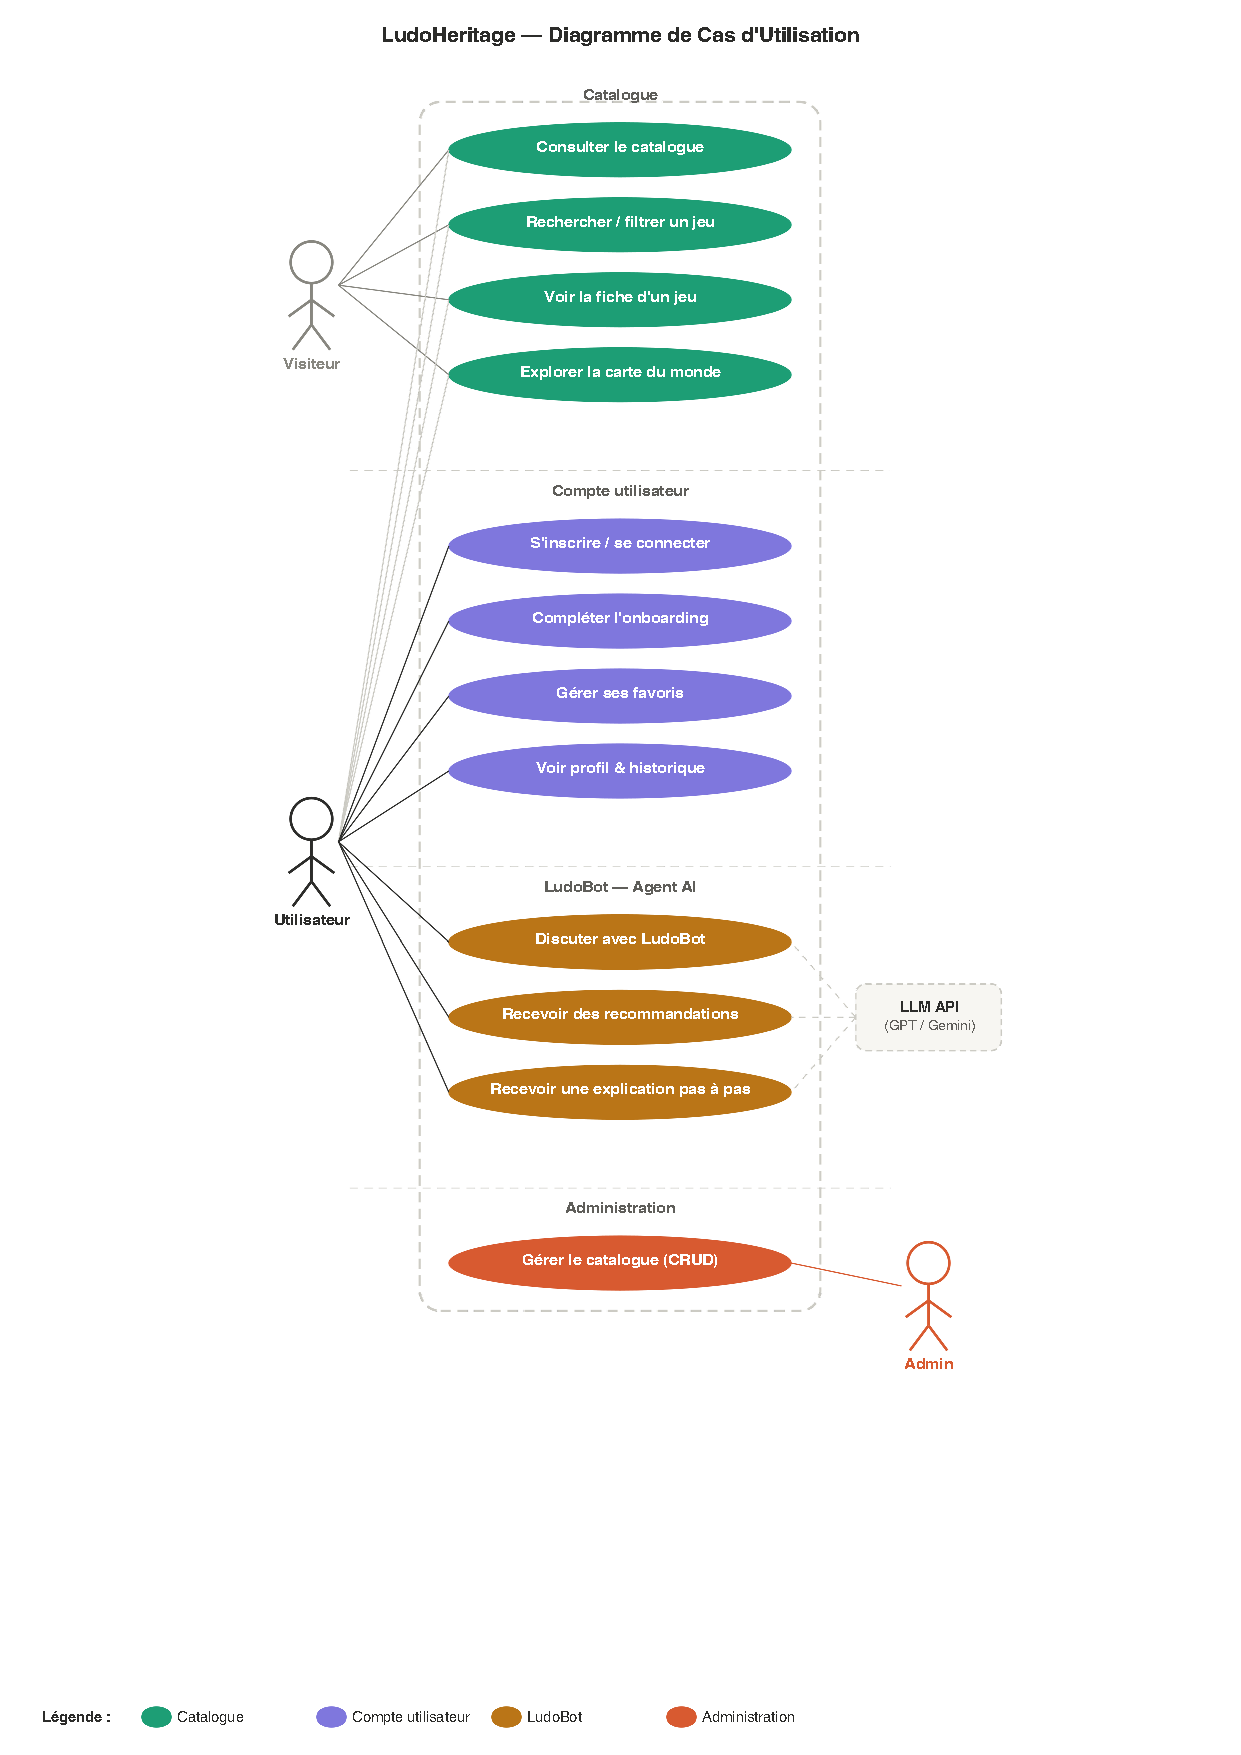
\includegraphics[width=\textwidth]{UML (1).pdf}
    \caption{Diagramme UML -- Structure du système LudoHeritage}
    \label{fig:uml-complet}
\end{figure}

\subsection{Modèle de cas d'utilisation détaillé}

Le modèle ci-dessous représente une vue exhaustive de tous les cas d'utilisation de la
plateforme, avec leurs relations d'inclusion et d'extension. Il complète le diagramme
général en montrant les dépendances entre chaque fonctionnalité.

\begin{figure}[H]
    \centering
    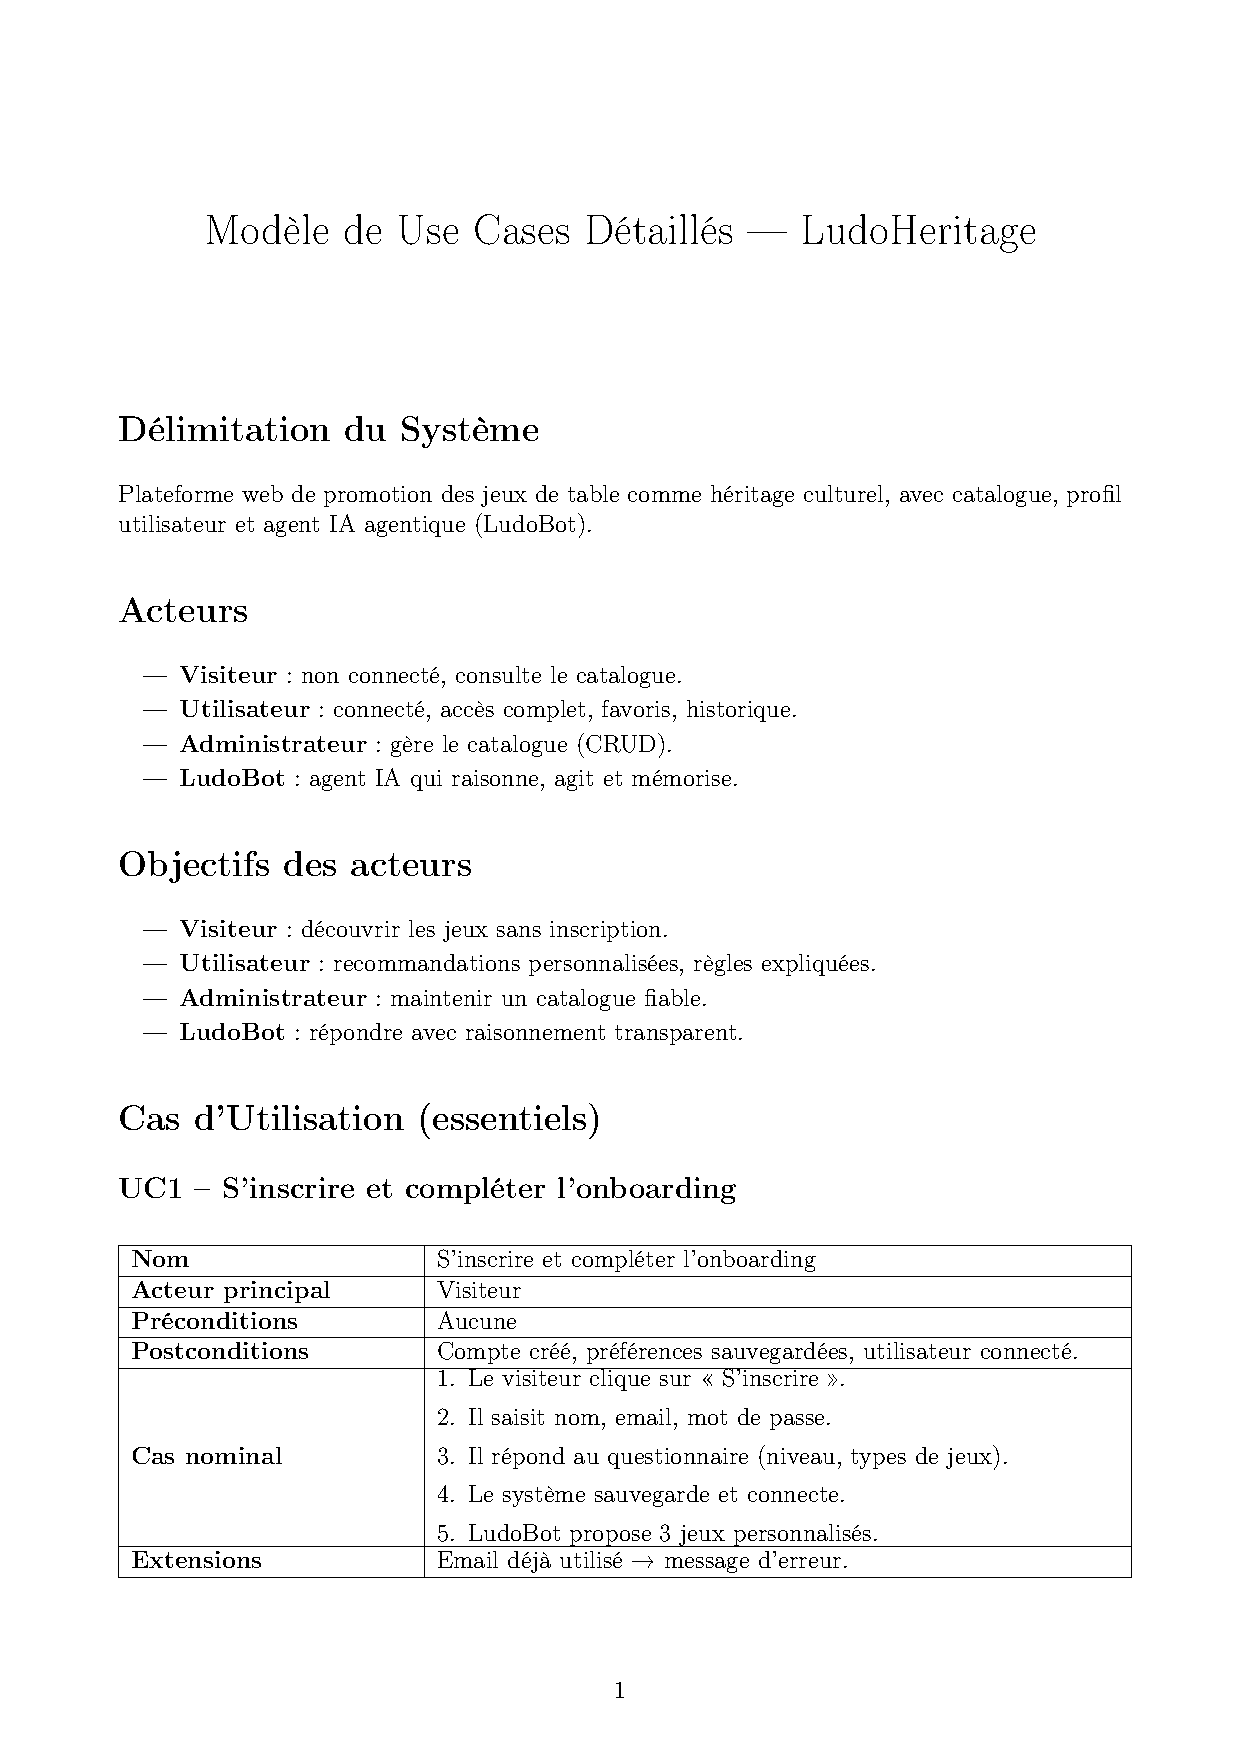
\includegraphics[width=\textwidth]{UseCase_ModelDetaillé (1).pdf}
    \caption{Modèle de cas d'utilisation détaillé -- LudoHeritage}
    \label{fig:usecase-detaille}
\end{figure}

% ─────────────────────────────────────────────────────────────────────────────
\section{Architecture du système}
% ─────────────────────────────────────────────────────────────────────────────

LudoHeritage adopte une architecture \textbf{trois-tiers} classique, séparant clairement
la présentation, la logique métier et la persistance des données.

\begin{figure}[H]
\centering
\renewcommand{\arraystretch}{2}
\begin{tabular}{|c|}
\hline
\textbf{Couche Présentation} \\
React 18 + Vite \quad \textbullet{} \quad SPA (Single Page Application) \\
Composants~: Catalogue, Carte, Chronologie, Quiz, Profil, LudoBot \\
\hline
$\updownarrow$ \quad Requêtes HTTP/REST (JSON) \\
\hline
\textbf{Couche Métier -- API REST} \\
Spring Boot 3.2 (Java 21) \\
Modules~: Auth, Jeux, Agent IA, Quiz, Communauté \\
LudoBot alimenté par \textbf{OllamaChatClient} (LLM local) \\
\hline
$\updownarrow$ \quad Spring Data MongoDB \\
\hline
\textbf{Couche Données} \\
MongoDB (collections~: users, games, quiz\_scores, community\_posts) \\
\hline
\end{tabular}
\caption{Architecture trois-tiers de LudoHeritage}
\label{fig:architecture}
\end{figure}

\subsection{Communication entre les couches}

\begin{itemize}
    \item Le frontend (React) communique avec le backend via des requêtes \textbf{HTTP REST},
          en envoyant et recevant des données au format \textbf{JSON}.

    \item Le backend expose plusieurs \textit{endpoints} organisés par domaine fonctionnel~:
          \texttt{/api/auth}, \texttt{/api/jeux}, \texttt{/api/agent}, \texttt{/api/quiz},
          \texttt{/api/community}.

    \item La gestion des accès croisés (\textbf{CORS}) est centralisée dans la classe
          \texttt{CorsConfig}, autorisant les requêtes depuis n'importe quelle origine en
          environnement de développement.

    \item \textbf{LudoBot} communique avec un modèle de langage installé localement via
          \textbf{Ollama} (port 11434). Le client \texttt{OllamaChatClient} interroge l'API
          \texttt{/api/generate} d'Ollama, en utilisant le premier modèle disponible ou celui
          configuré dans les propriétés de l'application.
\end{itemize}

% ─────────────────────────────────────────────────────────────────────────────
\section{Modèle de données}
% ─────────────────────────────────────────────────────────────────────────────

La base de données MongoDB est organisée autour de quatre collections principales~:

\begin{table}[H]
\centering
\renewcommand{\arraystretch}{1.4}
\begin{tabularx}{\textwidth}{>{\bfseries}p{3cm} p{4cm} X}
\toprule
\textbf{Collection} & \textbf{Champs principaux} & \textbf{Description} \\
\midrule
\texttt{users}
    & id, displayName, email, passwordHash, profile, onboardingCompleted, createdAt
    & Stocke les informations d'authentification et le profil de chaque utilisateur. \\
\midrule
\texttt{games}
    & id, name, region, country, period, type, difficulty, description, rules, history,
      ludemes, categories, reconstructionStatus, playable
    & Catalogue complet des 20 jeux traditionnels avec toutes leurs métadonnées culturelles. \\
\midrule
\texttt{community\_posts}
    & id, authorId, authorName, content, linkedGameId, linkedGameName, likeCount,
      comments, createdAt
    & Publications du forum communautaire avec système de likes et commentaires imbriqués. \\
\midrule
\texttt{quiz\_scores}
    & id, userId, displayName, score, total, playedAt
    & Scores des quiz soumis par les utilisateurs, utilisés pour le classement. \\
\bottomrule
\end{tabularx}
\caption{Collections MongoDB et leurs structures}
\label{tab:modele-donnees}
\end{table}

\subsection{Le modèle \texttt{Game} en détail}

L'entité centrale de l'application est le jeu traditionnel. Elle est représentée par un
\textit{record} Java immuable contenant~:

\begin{itemize}
    \item Les \textbf{métadonnées générales}~: nom, région, pays, période, type, difficulté,
          nombre de joueurs, durée.
    \item Les \textbf{contenus éducatifs}~: description, règles détaillées, histoire culturelle.
    \item Les \textbf{métadonnées académiques}~: statut de reconstruction, aliases connus,
          références, résumé des ludèmes (mécaniques de jeu).
    \item Les \textbf{étapes de tutoriel}~: liste de pas-à-pas avec des plateaux \og{}Avant/Après\fg{}
          illustrant chaque mouvement.
\end{itemize}

\subsection{Sélection des jeux}

Les vingt jeux ont été sélectionnés selon les critères suivants~:
\begin{enumerate}
    \item Représentativité géographique (Afrique, Asie, Europe, Amérique).
    \item Valeur historique et culturelle documentée.
    \item Absence de contenu associé à des pratiques contraires à l'éthique islamique
          (jeux de pari rituels, rites polythéistes).
    \item Diversité des mécaniques~: jeux de capture, de course, de territoire, de placement.
\end{enumerate}

% ─────────────────────────────────────────────────────────────────────────────
\section{Conception de l'interface utilisateur}
% ─────────────────────────────────────────────────────────────────────────────

\subsection{Principes directeurs}

La conception de l'interface de LudoHeritage s'est appuyée sur quatre principes fondamentaux~:

\begin{enumerate}
    \item \textbf{Clarté}~: chaque page a un objectif unique et clairement identifiable.
          La navigation par onglets (Catalogue, Carte, Chronologie, Ludèmes, Comparer, Quiz,
          Communauté, Profil) structure l'expérience sans confusion.

    \item \textbf{Élégance académique}~: la charte graphique s'inspire des portails de recherche
          (comme Ludii.games), avec des couleurs neutres (fond beige, encres foncées), une
          typographie Inter, et des cartes bordées sobres.

    \item \textbf{Cohérence}~: les composants réutilisables (cartes de jeu, badges de
          reconstruction, étiquettes de période) conservent le même aspect sur toutes les pages.

    \item \textbf{Progressivité}~: les fonctionnalités les plus simples (catalogue, carte) sont
          accessibles immédiatement. Les fonctionnalités avancées (quiz, comparaison) sont
          disponibles via la navigation.
\end{enumerate}

\subsection{Parcours utilisateur principal}

Le parcours typique d'un utilisateur se déroule comme suit~:

\begin{enumerate}
    \item \textbf{Inscription} ou \textbf{connexion} avec validation du mot de passe.
    \item \textbf{Onboarding}~: questionnaire de 4 questions pour personnaliser les recommandations.
    \item Exploration du \textbf{Catalogue} avec filtres ou de la \textbf{Carte mondiale}.
    \item Ouverture d'une fiche jeu via le modal tabulé (Aperçu, Règles, Histoire, Mécanique).
    \item Interaction avec \textbf{LudoBot} pour des questions complémentaires.
    \item Participation au \textbf{Quiz} et consultation du classement.
    \item Contribution au \textbf{Forum} ou ajout du jeu en favori.
    \item Consultation du \textbf{Profil} avec ses succès et recommandations personnalisées.
\end{enumerate}

% ─────────────────────────────────────────────────────────────────────────────
\section{Conclusion}
% ─────────────────────────────────────────────────────────────────────────────

Ce chapitre a présenté l'analyse complète des besoins de LudoHeritage et les choix de conception
qui en découlent. L'architecture trois-tiers, le modèle de données MongoDB et les principes de
conception de l'interface fournissent un cadre solide pour la réalisation. Le chapitre suivant
détaille la mise en œuvre technique de toutes ces fonctionnalités.
